% Author: Izaak Neutelings (December 2020)
% Sources:
%   https://commons.wikimedia.org/wiki/File:Punctuated-equilibrium.svg
%   https://thebrain.mcgill.ca/flash/capsules/outil_bleu09.html
\documentclass[border=3pt,tikz]{standalone}
\tikzset{>=latex} % for LaTeX arrow head
\usepackage{xcolor}
\colorlet{veccol}{green!45!black}
\colorlet{myred}{red!90!black}
\colorlet{myblue}{blue!90!black}
\colorlet{myorange}{orange!90!black}
\colorlet{mypurple}{blue!50!red!80!black!80}
\tikzstyle{tree}=[line cap=round,line join=round,line width=3,myorange]
\tikzset{mypos/.style={inner sep=0,outer sep=0,pos=#1}}
\usetikzlibrary{calc}

\begin{document}


% TWO VECTORS SUM
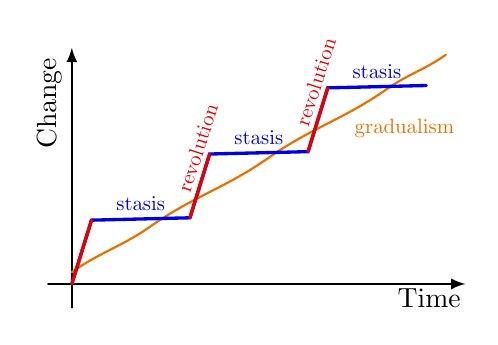
\begin{tikzpicture}[line cap=round] %[xscale=4,yscale=2]
  \def\xmax{5}
  \def\ymax{3}
  \def\xb{0.95*\xmax}
  \def\ya{0.05*\ymax}
  \def\yb{0.97*\ymax}
  \def\y#1{{\ya+(\yb-\ya)/(\xb)*#1}}
  \draw[->,thick] (-0.1*\ymax,0) -- (\xmax,0) node[below left=-2] {Time};
  \draw[->,thick] (0,-0.1*\ymax) -- (0,\ymax) node[above left,rotate=90] {Change};
  \draw[thick,myorange]
    (0,\ya)
      to[out=35,in=-145] (0.2*\xmax,\y{0.2*\xmax})
      to[out=35,in=-145] (0.5*\xmax,\y{0.5*\xmax})
      to[out=35,in=-145] (0.8*\xmax,\y{0.8*\xmax}) %node[below right,scale=0.75,myorange] {gradualism};
      to[out=35,in=-145] (\xb,\yb);
  \node[below right,scale=0.75,myorange] at (0.7*\xmax,\y{0.7*\xmax}) {gradualism};
  \draw[very thick,myblue]
    (0,0) coordinate (O) --++
    (0.05*\xmax,0.27*\ymax) coordinate (A1) --++
    (0.25*\xmax,0.01*\ymax) coordinate (A2) node[midway,above,scale=0.75] {stasis} --++
    (0.05*\xmax,0.27*\ymax) coordinate (B1) --++ %node[above,scale=0.5,rotate=60] {revolution} --++
    (0.25*\xmax,0.01*\ymax) coordinate (B2) node[midway,above,scale=0.75] {stasis} --++
    (0.05*\xmax,0.27*\ymax) coordinate (C1) --++ % node[above,scale=0.5,rotate=60] {revolution}
    (0.25*\xmax,0.01*\ymax) coordinate (C2) node[midway,above,scale=0.75] {stasis};
  \draw[very thick,myred]
    (O) -- (A1)
    (A2) node[left=3,above right=5,scale=0.75,rotate=72] {revolution} -- (B1)
    (B2) node[left=3,above right=5,scale=0.75,rotate=72] {revolution} -- (C1);
  
\end{tikzpicture}


% TREE - PHYLETIC GRADUALISM
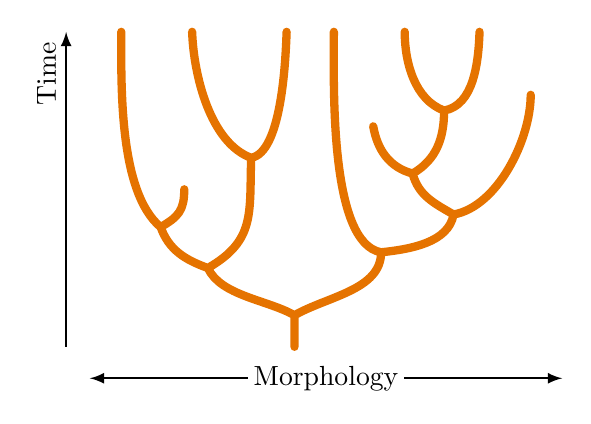
\begin{tikzpicture} %[x=1cm,y=0.4cm]
  
  % SETTINGS
  \def\xmax{3}
  \def\ymax{4}
  
  % COORDINATES
  \coordinate (A1) at (-0.4,0);
  \coordinate (A2) at (0.1,\ymax); % shift w.r.t. previous
  \coordinate (B1) at (-0.4,0.1*\ymax);
  \coordinate (B2) at (-0.5,\ymax);
  \coordinate (C1) at (-1.5,0.25*\ymax);
  \coordinate (C2) at (-2.6,\ymax);
  \coordinate (D1) at (-0.95,0.6*\ymax);
  \coordinate (D2) at (-1.7,\ymax);
  \coordinate (E1) at (-2.1,0.38*\ymax);
  \coordinate (E2) at (-1.8,0.5*\ymax);
  \coordinate (F1) at (0.7,0.3*\ymax);
  \coordinate (F2) at (1.0,\ymax);
  \coordinate (G1) at (1.62,0.42*\ymax);
  \coordinate (G2) at (2.6,0.8*\ymax);
  \coordinate (H1) at (1.1,0.55*\ymax);
  \coordinate (H2) at (0.6,0.7*\ymax);
  \coordinate (I1) at (1.5,0.75*\ymax);
  \coordinate (I2) at (1.95,\ymax);
  
  % TREE
  \draw[<->,thick] (-\xmax,-0.1*\ymax) --++ (2*\xmax,0)
    node[midway,fill=white,inner sep=2] {Morphology};
  \draw[->,thick] (-1.1*\xmax,0) --++ (0,\ymax)
    node[above left,rotate=90] {Time};
  \draw[tree]
    (A1) to[out=90,in=-90,looseness=1.2] (B1)
         to[out=30,in=-90,looseness=0.9] (F1)
         to[out=170,in=-90,looseness=0.6] (A2)
    (B1) to[out=150,in=-65,looseness=0.8] (C1)
         to[out=30,in=-92,looseness=1.2] (D1)
         to[out=10,in=-92,looseness=0.6] (B2)
    (F1) to[out=6,in=-100,looseness=0.9] (G1)
         to[out=150,in=-75,looseness=1.0] (H1)
         to[out=30,in=-90,looseness=1.0] (I1)
         to[out=160,in=-90,looseness=0.9] (F2)
    (C1) to[out=160,in=-70,looseness=1.0] (E1)
         to[out=140,in=-90,looseness=0.7] (C2)
    (D1) to[out=160,in=-88,looseness=0.8] (D2)
    (E1) to[out=30,in=-90,looseness=1.2] (E2)
    (G1) to[out=10,in=-90,looseness=0.8] (G2)
    (H1) to[out=165,in=-80,looseness=1.0] (H2)
    (I1) to[out=10,in=-92,looseness=0.9] (I2);
  
  %%%% HELP LINES & NODES
  %%%\draw[very thin,opacity=0.1] (-\xmax,0) grid[step=0.5] (\xmax,\ymax);
  %%%\draw[very thin,opacity=0.2] (-\xmax,0) grid[step=1.0] (\xmax,\ymax);
  %%%\foreach \p in {A1,A2,B1,B2,C1,C2,D1,D2,E1,E2,F1,F2,G1,G2,H1,H2,I1,I2}{
  %%%  \fill[opacity=0.3] (\p) circle(1pt) node[above right,scale=0.5] {\p};
  %%%}
  
\end{tikzpicture}


% TREE - PHYLETIC GRADUALISM
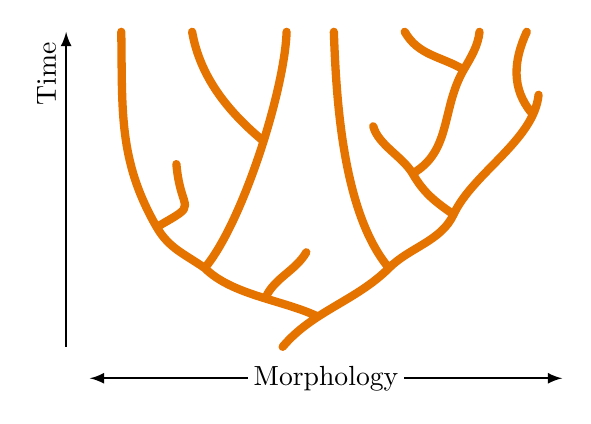
\begin{tikzpicture} %[x=1cm,y=0.4cm]
  
  % SETTINGS
  \def\xmax{3}
  \def\ymax{4}
  
  % COORDINATES
  \coordinate (A1) at (-0.55,0);
  \coordinate (A2) at (0.1,\ymax); % shift w.r.t. previous
  %\coordinate (B1) at (-0.4,0.1*\ymax);
  \coordinate (B2) at (-0.5,\ymax);
  \coordinate (C1) at (-1.54,0.25*\ymax);
  \coordinate (C2) at (-2.6,\ymax);
  %\coordinate (D1) at (-0.95,0.6*\ymax);
  \coordinate (D2) at (-1.7,\ymax);
  \coordinate (E1) at (-2.15,0.38*\ymax);
  \coordinate (E2) at (-1.9,0.58*\ymax);
  \coordinate (F1) at (0.8,0.25*\ymax);
  \coordinate (F2) at (1.0,\ymax);
  \coordinate (G1) at (1.62,0.42*\ymax);
  \coordinate (G2) at (2.7,0.8*\ymax);
  \coordinate (H1) at (1.1,0.55*\ymax);
  \coordinate (H2) at (0.6,0.7*\ymax);
  \coordinate (I1) at (1.75,0.88*\ymax);
  \coordinate (I2) at (1.95,\ymax);
  \coordinate (J2) at (-0.25,0.3*\ymax);
  \coordinate (K2) at (2.55,\ymax);
  
  % TREE
  \draw[<->,thick] (-\xmax,-0.1*\ymax) --++ (2*\xmax,0)
    node[midway,fill=white,inner sep=2] {Morphology};
  \draw[->,thick] (-1.1*\xmax,0) --++ (0,\ymax)
    node[above left,rotate=90] {Time};
  \draw[tree]
    (A1) to[out=50,in=-135,looseness=0.9]
         node[mypos=0.35] (B1) {} (F1)
         to[out=130,in=-88,looseness=0.75] (A2)
    (B1) to[out=155,in=-45,looseness=0.8]
         node[mypos=0.44] (J1) {} (C1)
         to[out=50,in=-92,looseness=0.6]
         node[mypos=0.55] (D1) {} (B2)
    (F1) to[out=45,in=-115,looseness=0.9] (G1)
         to[out=145,in=-60,looseness=1.0] (H1)
         to[out=30,in=-120,looseness=1.0] (I1)
         to[out=150,in=-60,looseness=1.0] (F2)
    (C1) to[out=145,in=-60,looseness=1.0] (E1)
         to[out=120,in=-89,looseness=1.0] (C2)
    (D1) to[out=140,in=-80,looseness=0.9] (D2)
    (E1) to[out=30,in=-85,looseness=2] (E2)
    (G1) to[out=65,in=-96,looseness=0.8]
         node[mypos=0.85] (K1) {} (G2)
    (H1) to[out=120,in=-75,looseness=0.8] (H2)
    (I1) to[out=60,in=-96,looseness=0.9] (I2)
    (J1) to[out=65,in=-120,looseness=0.9] (J2)
    (K1) to[out=130,in=-115,looseness=1.0] (K2);
  
  %%%% HELP LINES & NODES
  %%%\draw[very thin,opacity=0.1] (-\xmax,0) grid[step=0.5] (\xmax,\ymax);
  %%%\draw[very thin,opacity=0.2] (-\xmax,0) grid[step=1.0] (\xmax,\ymax);
  %%%\foreach \p in {A1,A2,B1,B2,C1,C2,D1,D2,E1,E2,F1,F2,
  %%%                G1,G2,H1,H2,I1,I2,J1,J2,K1,K2}{
  %%%  \fill[opacity=0.3] (\p) circle(1pt) node[above right,scale=0.5] {\p};
  %%%}
  
\end{tikzpicture}


% TREE - PUNCTUATED EQUILIBRIUM
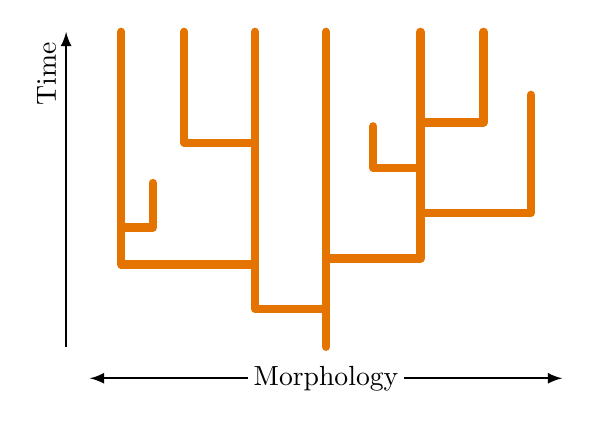
\begin{tikzpicture} %[x=1cm,y=0.4cm]
  
  % SETTINGS
  \def\xmax{3}
  \def\ymax{4}
  
  % COORDINATES
  \coordinate (A1) at (0,0);
  \coordinate (A2) at (0,\ymax);
  \coordinate (B2) at (-0.9,\ymax);
  \coordinate (C2) at (-2.6,\ymax);
  \coordinate (D2) at (-1.8,\ymax);
  \coordinate (E2) at (-2.2,0.52*\ymax);
  \coordinate (F2) at (1.2,\ymax);
  \coordinate (G2) at (2.6,0.8*\ymax);
  \coordinate (H2) at (0.6,0.7*\ymax);
  \coordinate (I2) at (2,\ymax);
  
  % TREE
  \draw[<->,thick] (-\xmax,-0.1*\ymax) --++ (2*\xmax,0)
    node[midway,fill=white,inner sep=2] {Morphology};
  \draw[->,thick] (-1.1*\xmax,0) --++ (0,\ymax)
    node[above left,rotate=90] {Time};
  \draw[tree]
    (A1) -- (A2)
    node[mypos=0.12] (B1) {}
    node[mypos=0.28] (F1) {}
    (B1) -| (B2)
    node[mypos=0.58] (C1) {}
    node[mypos=0.8] (D1) {}
    (F1) -| (F2)
    node[mypos=0.6] (G1) {}
    node[mypos=0.7] (H1) {}
    node[mypos=0.8] (I1) {}
    (C1) -| (C2)
    node[mypos=0.58] (E1) {}
    (D1) -| (D2)
    (E1) -| (E2)
    (G1) -| (G2)
    (H1) -| (H2)
    (I1) -| (I2);
  
  %%%% HELP LINES & NODES
  %%%\draw[very thin,opacity=0.1] (-\xmax,0) grid[step=0.5] (\xmax,\ymax);
  %%%\draw[very thin,opacity=0.3] (-\xmax,0) grid[step=1.0] (\xmax,\ymax);
  %%%\foreach \p in {A1,A2,B1,B2,C1,C2,D1,D2,E1,E2,F1,F2,G1,G2,H1,H2,I1,I2}{
  %%%  \fill[opacity=0.4] (\p) circle(1pt) node[above right,scale=0.5] {\p};
  %%%}
  
\end{tikzpicture}


% TREE - PUNCTUATED EQUILIBRIUM
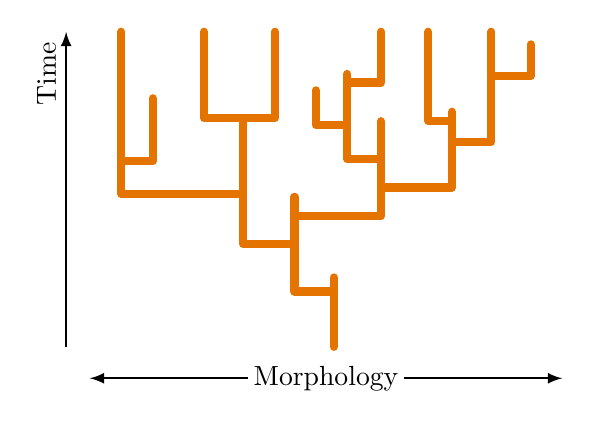
\begin{tikzpicture}[x=1cm,y=1cm]
  
  % SETTINGS
  \def\xmax{3}
  \def\ymax{4}
  
  % COORDINATES
  \coordinate (A1) at (0.1,0);
  \coordinate (C3) at (-0.65,\ymax);
  \coordinate (C4) at (-1.55,\ymax);
  \coordinate (E2) at (-2.6,\ymax);
  \coordinate (I2) at (0.7,\ymax);
  \coordinate (J2) at (1.3,\ymax);
  \coordinate (K2) at (2.1,\ymax);
  \coordinate (L2) at (2.6,0.96*\ymax);
  
  % TREE
  \draw[<->,thick] (-\xmax,-0.1*\ymax) --++ (2*\xmax,0)
    node[midway,fill=white,inner sep=2] {Morphology};
  \draw[->,thick] (-1.1*\xmax,0) --++ (0,\ymax)
    node[above left,rotate=90] {Time};
  \draw[tree]
    (A1) --++ (0,0.22*\ymax) coordinate(A2)
      node[mypos=0.8] (B1) {}
    (B1) -|++ (-0.5,0.3*\ymax) coordinate(B2)
      node[mypos=0.75] (C1) {}
      node[mypos=0.90] (D1) {}
    (C1) -|++ (-0.65,0.4*\ymax) coordinate(C2)
      node[mypos=0.7] (E1) {}
    (D1) -|++ (1.1,0.3*\ymax) coordinate(D2)
      node[mypos=0.65] (G1) {}
      node[mypos=0.80] (H1) {}
    (E1) -| (E2)
      node[mypos=0.6] (F1) {}
    (C2) -| (C3)
    (C2) -| (C4)
    (F1) -|++ (0.4,0.20*\ymax) coordinate(F2)
    (G1) -|++ (0.9,0.24*\ymax) coordinate(G2)
      node[mypos=0.94] (J1) {}
      node[mypos=0.8] (K1) {}
    (H1) -|++ (-0.43,0.27*\ymax) coordinate(H2)
      node[mypos=0.95] (I1) {}
      node[mypos=0.70] (M1) {}
    (I1) -| (I2)
    (J1) -| (J2)
    (K1) -| (K2)
      node[mypos=0.8] (L1) {}
    (L1) -| (L2)
    (M1) -|++ (-0.4,0.11*\ymax) coordinate(M2);
  
  %%%% HELP LINES & NODES
  %%%\draw[very thin,opacity=0.1] (-\xmax,0) grid[step=0.5] (\xmax,\ymax);
  %%%\draw[very thin,opacity=0.3] (-\xmax,0) grid[step=1.0] (\xmax,\ymax);
  %%%\foreach \p in {A1,A2,B1,B2,C1,C2,C3,C4,D1,D2,E1,E2,F1,F2,
  %%%                G1,G2,H1,H2,I1,I2,J1,J2,K1,K2,L1,L2,M1,M2}{
  %%%  \fill[opacity=0.4] (\p) circle(1pt) node[above right,scale=0.5] {\p};
  %%%}
  
\end{tikzpicture}


% TREE - PUNCTUATED EQUILIBRIUM (SLANTED)
% Slant the lines at small angle to indicate that there are
% still tiny changes over long periods of time (i.e. during stasis),
% although still smaller than in gradualism
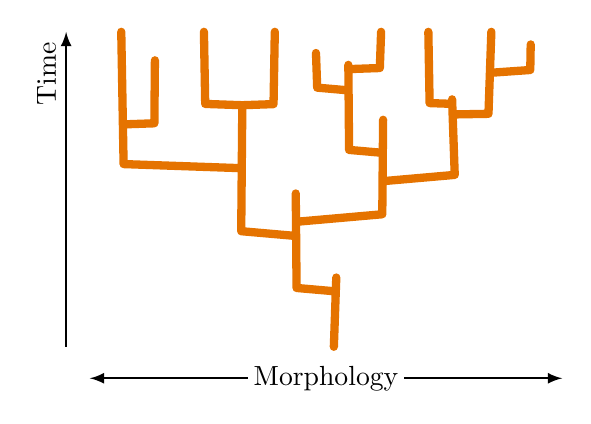
\begin{tikzpicture}[x=1cm,y=1cm]
  
  % SETTINGS
  \def\xmax{3}
  \def\ymax{4}
  
  % COORDINATES
  \coordinate (A1) at (0.1,0);
  \coordinate (C3) at (-0.65,\ymax);
  \coordinate (C4) at (-1.55,\ymax);
  \coordinate (E2) at (-2.6,\ymax);
  \coordinate (I2) at (0.7,\ymax);
  \coordinate (J2) at (1.3,\ymax);
  \coordinate (K2) at (2.1,\ymax);
  \coordinate (L2) at (2.6,0.96*\ymax);
  
  \def\branch(#1,#2)(#3){
    --++ (#1) --++ (90+#2*\ymax) coordinate(#3)
  }
  \def\branchend(#1:#2:#3:#4){
    coordinate(tmp#4) at ($(#1)!(#4)!($(#1)+(#2:0.1)$)$) % project
    (#1) -- ($(#4)!{sec(#3-#2)}!{#3-#2}:(tmp#4)$) -- (#4)
  }
  
  % TREE
  \draw[<->,thick] (-\xmax,-0.1*\ymax) --++ (2*\xmax,0)
    node[midway,fill=white,inner sep=2] {Morphology};
  \draw[->,thick] (-1.1*\xmax,0) --++ (0,\ymax)
    node[above left,rotate=90] {Time};
  \draw[tree]
    (A1) --++ (88:0.22*\ymax) coordinate(A2)
      node[mypos=0.8] (B1) {}
    (B1) \branch(175:0.5,0.5:0.3)(B2)
      node[mypos=0.55] (C1) {}
      node[mypos=0.70] (D1) {}
    (C1) \branch(175:0.7,-0.5:0.4)(C2)
      node[mypos=0.5] (E1) {}
    (D1) \branch(5:1.1,-0.5:0.3)(D2)
      node[mypos=0.35] (G1) {}
      node[mypos=0.65] (H1) {}
    \branchend(E1:178:1:E2)
      node[mypos=0.3] (F1) {}
    \branchend(C2:2:-1:C3)
    \branchend(C2:178:1:C4)
    (F1) \branch(2:0.40,-0.5:0.2)(F2)
    (G1) \branch(5:0.92,2:0.24)(G2)
      node[mypos=0.94] (J1) {}
      node[mypos=0.8] (K1) {}
    (H1) \branch(175:0.43,0.5:0.27)(H2)
      node[mypos=0.95] (I1) {}
      node[mypos=0.70] (M1) {}
    \branchend(I1:2:-2:I2)
    \branchend(J1:178:1:J2)
    \branchend(K1:1:-2:K2)
      node[mypos=0.5] (L1) {}
    \branchend(L1:4:-1:L2)
    (M1) \branch(175:0.4,2:0.11)(M2);
  
  %%%% HELP LINES & NODES
  %%%\draw[very thin,opacity=0.1] (-\xmax,0) grid[step=0.5] (\xmax,\ymax);
  %%%\draw[very thin,opacity=0.3] (-\xmax,0) grid[step=1.0] (\xmax,\ymax);
  %%%\foreach \p in {A1,A2,B1,B2,C1,C2,C3,C4,D1,D2,E1,E2,F1,F2,
  %%%                G1,G2,H1,H2,I1,I2,J1,J2,K1,K2,L1,L2,M1,M2}{
  %%%  \fill[opacity=0.4] (\p) circle(1pt) node[above right,scale=0.5] {\p};
  %%%}
  
\end{tikzpicture}



\end{document}